\documentclass[10pt]{article}  

%%%%%%%% PREÁMBULO %%%%%%%%%%%%
\title{Portada reporte practicas}
\usepackage[spanish]{babel} 
\usepackage[utf8]{inputenc}    
\usepackage{amsmath} 

%\usepackage{amssymb} 
\usepackage{graphicx} 
\usepackage{color} 
\usepackage{subfigure} 
\usepackage{float} 
\usepackage{capt-of} 
\usepackage{sidecap} 
	\sidecaptionvpos{figure}{c} 
\usepackage{caption} 
\usepackage{commath}  

\usepackage{cancel} 
 
\usepackage{anysize} 					
\marginsize{2cm}{2cm}{2cm}{2cm} 

\usepackage{appendix}
\renewcommand{\appendixname}{Apéndices}
\renewcommand{\appendixtocname}{Apéndices}
\renewcommand{\appendixpagename}{Apéndices} 

\usepackage[colorlinks=true,plainpages=true,citecolor=blue,linkcolor=blue]{hyperref}

\usepackage{fancyhdr} 
\pagestyle{fancy}
\fancyhf{}
\fancyhead[L]{\footnotesize UPIITA} 
\fancyhead[R]{\footnotesize IPN}   
\fancyfoot[R]{\footnotesize Programacion Avanzada}  
\fancyfoot[C]{\thepage} 
\fancyfoot[L]{\footnotesize Ing. Mecatrónica}  
\renewcommand{\footrulewidth}{0.4pt}


\usepackage{listings} 
\definecolor{dkgreen}{rgb}{0,0.6,0} 
\definecolor{gray}{rgb}{0.5,0.5,0.5} 

% configuración para el lenguaje que queramos utilizar
%\lstset{language=Matlab,
 %  keywords={break,case,catch,continue,else,elseif,end,for,function,
  %    global,if,otherwise,persistent,return,switch,try,while},
  % basicstyle=\ttfamily,
  % keywordstyle=\color{blue},
  % commentstyle=\color{red},
  % stringstyle=\color{dkgreen},
  % numbers=left,
  % numberstyle=\tiny\color{gray},
  % stepnumber=1,
  % numbersep=10pt,
  % backgroundcolor=\color{white},
   %tabsize=4,
   %showspaces=false,
   %showstringspaces=false}


\title{Plantilla portada}

%%%%%%%% TERMINA PREÁMBULO %%%%%%%%%%%%

\begin{document}

%%%%%%%%%%%%%%%%%%%%%%%%%%%%%%%%%% PORTADA %%%%%%%%%%%%%%%%%%%%%%%%%%%%%%%%%%%%%%%%%%%%
																					%%%
\begin{center}																		%%%
\newcommand{\HRule}{\rule{\linewidth}{0.5mm}}									%%%\left
 																					%%%
\begin{minipage}{0.48\textwidth} \begin{flushleft}

\includegraphics[scale = 0.63]{logo_upiita.png}
\end{flushleft}\end{minipage}
\begin{minipage}{0.48\textwidth} \begin{flushright}

\includegraphics[scale = 0.35]{IPN.jpg}
\end{flushright}\end{minipage}

													 								%%%
\vspace*{-1.5cm}								%%%
																					%%%	
\textsc{\huge Instituto Polit\'ecnico\\ \vspace{5px} Nacional}\\[1.5cm]	

\textsc{\LARGE Unidad Profesional Interdisciplinaria en Ingenier\'ia y				%%%
Tecnolog\'ias Avanzadas}\\[1.5cm]													%%%

\begin{minipage}{0.9\textwidth} 
\begin{center}																					%%%
\textsc{\LARGE Programación Avanzada 2MV7}
\end{center}
\end{minipage}\\[0.5cm]
%%%
    																				%%%
 			\vspace*{1cm}																		%%%
																					%%%
\HRule \\[0.4cm]																	%%%
{ \huge \bfseries Practica 0}\\[0.4cm]	%%%
 																					%%%
\HRule \\[1.5cm]																	%%%
 																				%%%
																					%%%
\begin{minipage}{0.46\textwidth}													%%%
\begin{flushleft} \large															%%%
\emph{Autor:}\\	
Barrios Mendez Jose Alberto\\
Boleta: 2022640111


%%%
			%\vspace*{2cm}	
            													%%%
										 						%%%
\end{flushleft}																		%%%
\end{minipage}		
																%%%
\begin{minipage}{0.52\textwidth}		
\vspace{-0.6cm}											%%%
\begin{flushright} \large															%%%
\emph{Profesor:} \\																	%%%
Cruz Mora Jose Luis\\
													%%%
\end{flushright}																	%%%
\end{minipage}	
\vspace*{1cm}
%\begin{flushleft}
 	
%\end{flushleft}
%%%
 		\flushleft{\textbf{\Large Ing. Mecatrónica}	}\\																		%%%
\vspace{2cm} 																				
\begin{center}																					
{\large \today}																	%%%
 			\end{center}												  						
\end{center}							 											
																					
\newpage																		
%%%%%%%%%%%%%%%%%%%% TERMINA PORTADA %%%%%%%%%%%%%%%%%%%%%%%%%%%%%%%%

\tableofcontents 

\newpage

\section{Objetivo.}

Realizar la instalacíon del software que se utilizara en el curso, ası como conocer y practicar la forma de trabajo.



\section{Introduccion.} 

En esta practica analizaremos la forma en la cual podemos escribir un programa de forma sencilla en el lenguaje de programacion Python

\section{Desarrollo.}
Para el desarrollo de esta practica unicamente necesitamos conocer la sintexis para poder imprimir un mensaje en la consola de salida, solo debemos implementar dicha sintaxis y el programa estara terminado


\section{Ejecucion.}

\begin{figure}[H]
	\begin{center}
 		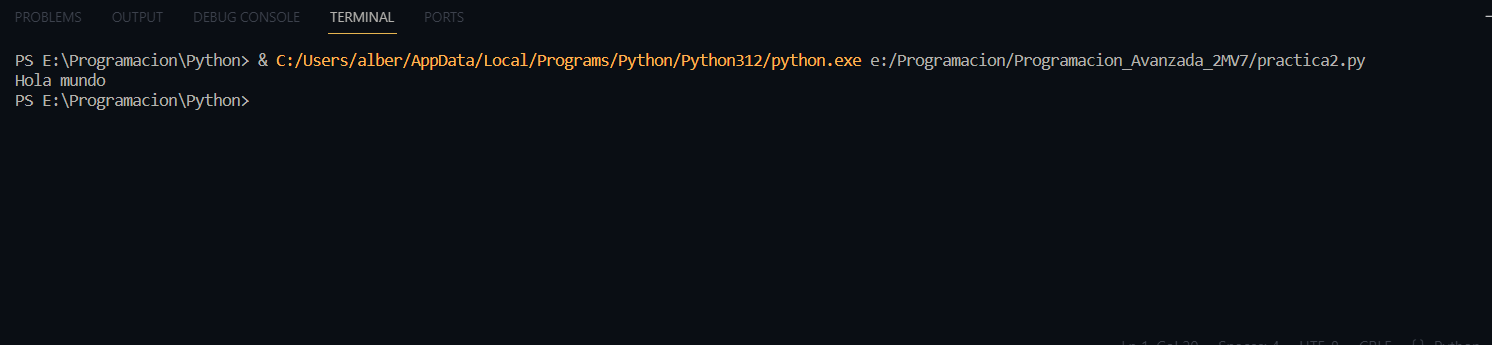
\includegraphics[width = 1\textwidth]{ejecucion.png}
 		\captionof{figure}{\label{fig:IPN}Hola mundo en python (resultado en consola)} 
	\end{center} 
\end{figure}





\section{Conclusiones.}
Para concluir, debemos reconocer que iniciar con un nuevo lenguaje de programacion es todo una experencia, sin embargo al comparar con algunos otros lenguajes como C/C++, esta sintaxis es bastante sencilla en comparacion de los lenguajes con los que anteriormente habia trabajado
\
%%%%%%% Bibliografía %%%%%%%%    

%\appendix  
%\clearpage % o \cleardoublepage
%\addappheadtotoc 
%\appendixpage

%\section{Anexos 1.}




%\section{Anexos 2.}


 

\end{document}
